\documentclass[11pt,a4paper]{article}

\usepackage[utf8]{inputenc}
\usepackage[T1]{fontenc}
\usepackage[left=2.5cm, right=2.5cm, top=2.5cm, bottom=2.5cm]{geometry}
\usepackage{amsmath, amssymb, amsthm}
\usepackage{graphicx}
\usepackage{booktabs}
\usepackage{tabularx}
\usepackage[justification=raggedright, singlelinecheck=false, skip=0pt]{caption}
\usepackage{titlesec}
\usepackage{enumitem}
\usepackage{xcolor}
\usepackage[left]{authblk}
\usepackage{lineno}
\usepackage{float}
\usepackage{fancyhdr}
\usepackage{hyperref}
\usepackage[numbers,sort&compress]{natbib}

\linenumbers

\pagestyle{fancy}
\fancyhf{}
\renewcommand{\headrulewidth}{0pt}
\fancyfoot[L]{\small APBC2026}
\fancyfoot[R]{\thepage}

\captionsetup{
    labelfont       = bf,
    labelsep        = period,
    justification   = raggedright,
    singlelinecheck = false,
    skip            = 0pt
}

\renewcommand\Affilfont{\small}

\renewenvironment{abstract}
  {\noindent\small\textbf{Abstract:}\enspace}
  {\par}

\newcommand{\keywords}[1]{
  \noindent\begin{flushleft}\small\textbf{Keywords:}\enspace #1\end{flushleft}
  \nointerlineskip
  \noindent\rule{\textwidth}{0.8pt}
  \vskip 2em
}

\makeatletter
\renewcommand{\maketitle}{
  \begin{flushleft}
    \nointerlineskip
    \noindent\rule{\textwidth}{0.8pt}
    {\huge \bfseries \@title \par}
    \vskip 2em
    {\@author \par}
    \vskip 1.5em
  \end{flushleft}
}

\renewenvironment{proof}[1][\proofname]{\par
  \pushQED{\qed}%
  \normalfont \topsep6\p@\@plus6\p@\relax
  \trivlist
  \item[\hskip\labelsep \bfseries #1\@addpunct{.}]\ignorespaces
}{%
  \popQED\endtrivlist\@endpefalse
}
\makeatother

\renewenvironment{abstract}
  {\noindent\small\textbf{Abstract:}\enspace}
  {\par\vskip 1em}

\newcommand{\keywords}[1]{
  \noindent\begin{flushleft}\textbf{Keywords:}\enspace #1\end{flushleft}
  \nointerlineskip
  \noindent\rule{\textwidth}{0.8pt}
  \vskip 2em
}

\theoremstyle{plain}
\newtheorem{theorem}{Theorem}
\newtheorem{proposition}[theorem]{Proposition}
\newtheorem{lemma}[theorem]{Lemma}

\theoremstyle{definition}
\newtheorem{remark}{Remark}
\newtheorem{example}{Example}

\titleformat{\section}{\normalfont\large\bfseries}{\thesection.}{0.5em}{}
\titlespacing{\section}{0pt}{3.5ex plus 1ex minus .2ex}{0.5ex}

\titleformat{\subsection}{\normalfont\normalsize\itshape}{\thesubsection.}{0.5em}{}
\titlespacing{\subsection}{0pt}{2ex plus 0.5ex minus .2ex}{0.1ex}

\titleformat{\subsubsection}{\normalfont\normalsize}{\thesubsubsection.}{0.5em}{}
\titlespacing{\subsubsection}{0pt}{0.5ex plus 0.2ex minus .1ex}{0.1ex}

\title{DELTA: A Gain-Loss Decomposition Framework for Interpretable Protein Stability Prediction}
\author[1,*]{\textbf{A Shivram}}
\author[1]{\textbf{Aneesh S. Chivukula}}
\author[1]{\textbf{Manik Gupta}}
\author[2,*]{\textbf{Sourav Chowdhury}}
\affil[1]{Department of Computer Science and Information Systems, Birla Institute of Technology and Science Pilani, Hyderabad Campus, Telangana, India}
\affil[2]{Department of Biological Sciences, Birla Institute of Technology and Science Pilani, Hyderabad Campus, Telangana, India}
\affil[*]{Correspondence: p20230075@hyderabad.bits-pilani.ac.in}
\vskip 1em
\date{}

\begin{document}

\maketitle
\thispagestyle{fancy}

\begin{abstract}
Predicting the effect of amino acid substitutions on protein thermodynamic stability is a fundamental problem in protein engineering, molecular evolution, and clinical variant interpretation. Recent deep learning models achieve strong predictive performance for mutation-induced stability changes ($\Delta\Delta G$), yet almost universally produce a single scalar output that provides little insight into the mechanistic factors underlying a prediction. Here, we introduce DELTA, a structure-aware framework that models mutation effects through an explicit gain--loss decomposition. DELTA combines multimodal residue representations derived from ProteinMPNN and ESM-2 with mutation-type conditioning and separate gain and loss branches, trained solely using experimentally measured $\Delta\Delta G$ values and anti-symmetry-based consistency constraints. No component-level supervision, physical annotations, or mechanistic labels are provided during training. Across multiple protein stability benchmarks, DELTA achieves predictive performance comparable to a strong single-output baseline while exposing an interpretable latent decomposition. Analysis of the learned components reveals strong reverse-direction consistency between forward and reverse mutations, systematic dependence on mutation type, and reproducible relationships with structural context, including residue burial. These properties emerge despite never being specified as training targets and remain observable across multiple architectural variants. The results demonstrate that a mechanistically consistent gain-loss structure can be recovered from standard $\Delta\Delta G$ supervision without sacrificing predictive accuracy. More broadly, this work reframes protein stability prediction as a latent decomposition problem and provides a diagnostic framework for evaluating whether biologically meaningful mechanistic structure emerges from supervised learning in the absence of component-level labels.
\end{abstract}

\keywords{protein stability prediction;
mutation effect prediction;
protein language models;
multimodal representation learning;
interpretable deep learning;
latent decomposition;
computational biology
}

\section{Introduction}
The effect of mutation on protein thermodynamic stability is a central determinant of protein function, evolvability, and disease. Changes in folding free energy ($\Delta\Delta G$) influence whether a protein adopts and maintains its native structure, making accurate stability prediction a foundational problem in protein engineering, antibody optimization, and clinical variation interpretation. Recent advances in protein language models and structure-aware neural networks have substantially improved predictive performance, enabling large-scale estimation of mutation effects across diverse protein families~\cite{lin2023evolutionary,dauparas2022robust,rives2021biological}. Despite these advances, most contemporary predictors share a common characteristic: they map a mutation directly to a single scalar stability value.

This formulation has been remarkably successful for prediction, but it leaves an important scientific question unanswered. A predicted $\Delta\Delta G$ quantifies the net effect of a mutation without explaining the underlying factors that produced it. A destabilizing mutation may arise from the loss of a favorable hydrophobic packing, disruption of the hydrogen-bond network, introduction of steric clashes, altered electrostatic interactions, or a combination of multiple mechanisms. Distinct molecular processes can therefore produce similar stability changes, making the scalar prediction difficult to interpret and limiting its usefulness for rational protein redesign. For many applications, understanding \emph{why} a mutation is predicted to alter stability is nearly as important as estimating \emph{how much} it alters stability.

A natural view of mutation effects is decompositional: replacing a residue simultaneously removes existing interactions and introduces new ones. From this perspective, the observed $\Delta\Delta G$ can be interpreted as the balance between a contribution lost from the wild-type residue and a contribution gained from the mutant residue. However, only the net $\Delta\Delta G$ is experimentally observable, creating an identifiability problem in which many different gain--loss decompositions can explain the same measurement. A model could therefore achieve excellent predictive accuracy while assigning arbitrary values to its latent components. Predictive performance alone is thus insufficient to establish whether a learned decomposition reflects meaningful biological structure or merely a convenient mathematical factorization, motivating the need for independent tests of decomposition consistency.

We introduce DELTA, a structure-aware framework that models mutation-induced stability changes through an explicit gain-loss decomposition conditioned on residue identity, mutation type, and local structural context. DELTA is trained solely on experimentally measured $\Delta \Delta G$ values together with symmetry-based consistency constraints; no component-level labels, physical annotations, or mechanistic supervision are provided. Because gain and loss are latent quantities for which no experimental measurements exist, the critical challenge is not fitting observed stability changes but rather determining whether the learned decomposition exhibits consistent, biologically interpretable, and structurally grounded behavior. DELTA addresses this challenge by directly learning decomposition from standard $\Delta\Delta G$ supervision and evaluating its consistency through independent diagnostic analyses.

To evaluate whether the learned decomposition is meaningful, we perform a series of independent analyses on held-out mutations. Specifically, we examine consistency under mutation reversal, the behavior of conservative versus non-conservative substitutions, associations with structural context, and the robustness of the decomposition across architectural variants. Together, these analyses test whether the learned components exhibit coherent biological and structural behavior beyond what would be expected from an arbitrary factorization of the prediction.

Our principal finding is that a mechanistically consistent gain-loss decomposition emerges despite the absence of component-level supervision. The learned components exhibit strong reverse-direction consistency, respond systematically to mutation type, show reproducible relationships with structural context, and remain stable across multiple architectural variants. Importantly, these properties are not imposed through explicit physical labels but arise from information contained in the $\Delta\Delta G$ prediction task itself. These results suggest that mutation effect predictors can recover latent mechanistic structure while maintaining competitive predictive accuracy.

The main contributions of this work are:
\begin{itemize}
\item \textbf{A latent decomposition formulation for protein stability prediction.}
We reformulate mutation-effect prediction as the recovery of latent gain and loss components from observed $\Delta\Delta G$ measurements and explicitly address the associated identifiability challenge.
\item \textbf{DELTA, a decomposition-based stability predictor.}
We introduce DELTA, a structure-aware framework that models mutation effects through gain and loss components conditioned on residue identity, mutation type, and local structural context, without requiring component-level supervision.
\item \textbf{A diagnostic framework for evaluating latent decompositions.}
We develop a suite of independent consistency tests, including reverse-consistency, conservative-substitution attenuation, structural-context association, and embedding-directionality analyses, to assess whether learned decompositions exhibit biologically meaningful behavior.
\item \textbf{Evidence for emergent mechanistic structure.}
We demonstrate that a mechanistically consistent gain--loss structure emerges from standard $\Delta\Delta G$ supervision alone and remains stable across multiple architectural realizations, suggesting that mutation-effect predictors can recover latent mechanistic information without explicit physical annotation.
\end{itemize}

\section{Related Work}
\subsection{Protein stability prediction}
Predicting mutation-induced changes in protein stability ($\Delta\Delta G$) is a fundamental problem in protein engineering, molecular evolution, and variant interpretation. Early approaches relied primarily on physics-based energy functions, including FoldX~\cite{schymkowitz2005foldx} and Rosetta~\cite{leaver2011rosetta3}, which estimate the energetic consequences of a mutation through explicit modeling of molecular interactions such as packing, electrostatics, hydrogen bonding and solvation. These methods provide physically interpretable energy terms but remain limited by force-field approximations and often require substantial computation.

The success of deep learning has shifted the field toward data-driven predictors. Methods such as DeepDDG~\cite{cao2019deepddg}, ThermoNet~\cite{li2020predicting}, DDMut~\cite{zhou2023ddmut}, ThermoMPNN~\cite{dieckhaus2024transfer}, RaSP~\cite{blaabjerg2023rapid}, and more recent protein-language-model (PLM)- based approaches learn statistical relationships between sequences, structures, and experimentally measured stability changes~\cite{rives2021biological,brandes2022proteinbert,ofer2021language,lin2023evolutionary}. The introduction of large PLM and inverse folding architectures~\cite{dauparas2022robust} has further improved predictive performance by enabling rich contextual representations of both sequence and structure. Recent multimodal frameworks, including SPURS~\cite{li2025generalizable}, combine language-model embeddings with structure-aware representations and achieve strong performance across standard stability benchmarks.

Despite substantial architectural diversity, most contemporary predictors share a common formulation: a mutation is mapped directly to a single scalar $\Delta\Delta G$. Progress is therefore measured primarily through improvements in correlation and error metrics. Comparatively little attention has been devoted to whether the prediction itself contains recoverable mechanistic structure beyond the final scalar output.

\subsection{Thermodynamic consistency and direction-aware prediction}
A fundamental physical property of mutation-induced stability change is anti-symmetry,
\[
\Delta\Delta G(a \rightarrow b) = -\Delta\Delta G(b \rightarrow a),
\]
which follows directly from thermodynamic reversibility. However, unconstrained machine learning models frequently violate this property, motivating the development of thermodynamically consistent architectures.

Several methods explicitly incorporate anti-symmetry into model design or training. Thermodynamic cycle-based approaches enforce consistency between forward and reverse mutations through architectural constraints. ACDC-NN~\cite{benevenuta2021antisymmetric} and related models introduce anti-symmetric neural formulations that satisfy thermodynamic requirements by construction. More recently, JanusDDG~\cite{barducci2026janusddg} combines protein-language-model representations with bidirectional modeling and thermodynamic constraints to improve consistency across mutation directions.

These methods demonstrate the importance of respecting physical symmetries during prediction. Nevertheless, their objective remains to predict a single scalar stability change. Anti-symmetry is used to constrain or improve the prediction itself rather than to recover latent mechanistic factors underlying that prediction. In contrast, DELTA employs anti-symmetry as an inductive bias for learning and evaluating a gain-loss decomposition of mutation effects.

\subsection{Interpretability in mutation-effect prediction}

Interpretability remains a major challenge for modern mutation-effect predictors.

It consists of post-hoc explanation methods, including gradient-based attribution~\cite{selvaraju2017grad}, integrated gradients~\cite{sundararajan2017axiomatic}, attention visualization~\cite{vaswani2017attention,chen2021attention}, and SHAP-style feature attribution~\cite{lundberg2017unified}. These approaches identify which inputs most influence a prediction but do not explicitly model the underlying mechanisms responsible for stability change. As a result, explanations are tied to individual predictions and may not correspond to reusable biological concepts.

DELTA occupies a different position. Rather than applying post-hoc explanations to a scalar prediction or imposing predefined physical terms, it learns a latent gain-loss decomposition directly from $\Delta\Delta G$ supervision and subsequently evaluates whether the learned components exhibit biologically meaningful behavior. The objective is not to recover known energy terms but to determine whether a mechanistically consistent structure emerges from the prediction task itself.

\subsection{Latent decomposition and identifiability}

The central challenge addressed by DELTA is closely related to the broader problem of latent-variable identifiability. When only an aggregate quantity is observed, many latent factorizations may explain the same measurement. Consequently, predictive accuracy alone cannot establish whether a learned decomposition is meaningful.

This problem has been studied extensively in representation learning~\cite{bengio2013representation}, disentangled representation learning~\cite{kim2018disentangling}, matrix factorization, and latent-variable modeling. Common approaches introduce additional constraints, auxiliary supervision, sparsity assumptions, invariance principles, or structured priors to encourage interpretable latent factors. The underlying lesson is that latent variables are meaningful only to the extent that they exhibit consistent behavior under independent evaluation.

Protein stability prediction presents a particularly challenging instance of this problem because experiments provide only the net $\Delta\Delta G$ and offer no direct measurements of gain and loss components. Any proposed decomposition is therefore inherently underdetermined. Rather than claiming to recover a unique or physically exact factorization, DELTA addresses this challenge through architectural separation, mutation-type conditioning, thermodynamic consistency constraints, and a suite of independent diagnostics designed specifically to evaluate whether the learned decomposition exhibits reproducible biological and structural regularities.

In summary, prior work has focused either on improving scalar $\Delta\Delta G$ prediction, enforcing thermodynamic consistency, or explaining predictions through post-hoc analyses. DELTA addresses a different question: whether biologically meaningful gain and loss components can emerge from standard $\Delta\Delta G$ supervision despite the absence of component-level labels. The proposed diagnostic framework provides a means to directly evaluate this question.

\section{Methods}
\label{sec:methods}

\subsection{Problem formulation and decomposition principle}
Let a wild-type protein be given by its sequence $S = (s_1,\dots,s_L)$ and
backbone coordinates $X \in \mathbb{R}^{L\times 4 \times 3}$ (atoms
$\mathrm{N}, \mathrm{C}\alpha, \mathrm{C}, \mathrm{O}$). A single-point
mutation is the triple $(i, a, b)$: position $i$, wild-type residue
$a = s_i$, mutant residue $b$. The task is to predict the scalar $\Delta\Delta G$.
DELTA computes
\begin{equation}
\widehat{\Delta\Delta G}(i, a\!\rightarrow\!b) \;=\; g_\theta(b \mid \mathcal{C}_i) \;-\; \ell_\theta(a \mid \mathcal{C}_i),
\label{eq:decomp2}
\end{equation}
where $\mathcal{C}_i$ is a representation of the structural environment of
site $i$, and $g_\theta, \ell_\theta : \mathbb{R} \rightarrow \mathbb{R}$
are scalar-valued gain and loss branches. The two branches are combined
only by the final subtraction; the gain and loss values are never
individually supervised (Section~\ref{sec:objective}).
\begin{figure}
    \centering
    \includegraphics[width=1\linewidth]{figures/fig_1.pdf}
    \caption{Overview of DELTA. ProteinMPNN and ESM-2 representations are fused through cross-attention to produce residue-level representations. A structural context encoder constructs a mutation-site representation conditioned on mutation-type and residue-identity embeddings. Separate gain and loss branches estimate the contributions gained by introducing the mutant residue and lost by removing the wild-type residue, respectively. Their difference yields the final predicted $\Delta\Delta G$. DELTA-B replaces the shared-context formulation with identity-conditioned attention queries.}
    \label{fig:architecture}
\end{figure}
\subsection{Backbone representation}
\label{sec:backbone}

We obtain per-residue representations from a multimodal backbone that integrates structural information from an inverse-folding encoder with evolutionary representations from a protein language model. Structural features are extracted using ProteinMPNN, sequence representations are obtained from ESM-2, and the two modalities are fused through cross-attention to generate context-aware residue embeddings. These representations form the input to the DELTA decomposition module and are also used to construct a single-output baseline for comparison. An overview of the complete architecture is shown in Figure~\ref{fig:architecture}.

Specifically, an inverse-folding encoder ProteinMPNN~\cite{dauparas2022robust} processes $(X,S)$ and yields, for each residue, the concatenation of its hidden node features, sequence embedding, and intermediate message-passing states, producing a structural representation of dimension $d_{\mathrm{enc}}$. In parallel, ESM-2 (650M parameters, 33 layers~\cite{lin2023evolutionary} equipped with a structural adapter consumes the amino-acid sequence while incorporating encoder-derived structural information injected at the adapter layer. The resulting contextual sequence representations have dimension $1280$.

The structural and sequence streams are integrated through a multi-head cross-attention module (embedding dimension $1280$, $8$ attention heads), using ESM-2 representations as queries and ProteinMPNN features as keys and values. The fused representation is concatenated with the structural encoder output to obtain the final per-residue embedding
\begin{equation}
H \in \mathbb{R}^{T \times d}, \qquad d = 1280 + d_{\mathrm{enc}} = 1408,
\end{equation}
which serves as the input to the DELTA decomposition modules described below.

\subsection{Mutation-type and residue-identity embeddings}
\label{sec:embeddings}

Both branches are conditioned on the chemistry and directionality of the substitution. To represent mutation-specific information, we maintain a learned \emph{mutation-type embedding} $E \in \mathbb{R}^{20 \times 20 \times d_{\mathrm{sub}}}$ with $d_{\mathrm{sub}} = 64$, indexed by the ordered amino-acid pair $(a, b)$, where (a) denotes the wild-type residue and (b) the mutant residue. Thus, $E_{a,b}$ encodes the directed substitution $a\!\rightarrow\!b$, allowing the model to distinguish, for example $A\!\rightarrow\!V$ from $V\!\rightarrow\!A$.

To incorporate biologically meaningful prior information, the first latent channel of $E$ is initialized from the mean-centered, unit-variance BLOSUM62 substitution matrix~\cite{henikoff1992amino}, while the remaining channels are initialized from $\mathcal{N}(0,0.02^2)$. This initialization places evolutionarily similar substitutions close together in the initial embedding space while preserving sufficient flexibility for the model to learn task-specific and directional relationships during training.

In addition to substitution-level information, we introduce a separate
\emph{residue-identity} embedding
$U \in \mathbb{R}^{20 \times d_{\mathrm{aa}}}$ with
$d_{\mathrm{aa}} = 64$, initialized using Xavier initialization. For an
amino acid $a$, we denote its embedding by $u_a = U_a$.

The mutation-type embedding and the residue-identity embeddings serve complementary roles. The mutation-type embedding $E_{a,b}$ captures properties specific to the substitution itself, such as conservative versus non-conservative exchanges or hydrophobic-to-charged transitions. In contrast, the residue-identity embeddings provide branch-specific conditioning, enabling the gain and loss branches to reason independently about the introduced and removed residues.

Accordingly, the mutant identity embedding $u_b$ conditions the gain branch, whereas the wild-type identity embedding $u_a$ conditions the loss branch. This design explicitly aligns the architectural decomposition with the biological interpretation of mutation effects: the gain branch models contributions associated with introducing residue $b$, while the loss branch models contributions associated with removing residue $a$.

\subsection{Structural context encoder}
\label{sec:context}

The context $\mathcal{C}_i$ is computed by distance-modulated multi-head
attention over the spatial neighborhood of site $i$. Using $\mathrm{C}\alpha$
coordinates, we form the pairwise distance matrix $D \in \mathbb{R}^{L\times L}$
and select, for the mutation site, its $k = 32$ nearest neighbors
$\mathcal{N}(i)$ (excluding $i$ and any masked residues). Let
$h_i \in \mathbb{R}^{d}$ be the site representation (row $i+1$ of $H$) and
$\{h_j\}_{j\in\mathcal{N}(i)}$ the neighbor representations. With $n_h = 8$
heads of dimension $d_h = d / n_h = 176$, head $m$ computes a query from the
site, and keys/values from the neighbors:
\begin{equation}
q^{(m)} = W_Q^{(m)} \tilde{h}_i, \quad
k_j^{(m)} = W_K^{(m)} h_j, \quad
v_j^{(m)} = W_V^{(m)} h_j .
\end{equation}
Attention weights combine the scaled dot product with a learned Gaussian
distance kernel and a learned distance bias. For neighbor $j$ at distance
$D_{ij}$,
\begin{equation}
\alpha^{(m)}_{ij} \;\propto\; \exp\!\Big(\tfrac{q^{(m)\top} k_j^{(m)}}{\sqrt{d_h}}\Big)
\cdot \underbrace{\exp\!\Big(-\tfrac{D_{ij}^2}{2\sigma_m^2}\Big)}_{\text{distance kernel}}
\;+\; \beta_m(D_{ij}),
\label{eq:attn}
\end{equation}
where the per-head length scale $\sigma_m$ is a learned parameter
(initialized at $8.0$\,\AA, stored as $\log\sigma_m$ for positivity) and
$\beta_m(\cdot)$ is a two-layer MLP mapping a scalar distance to a per-head
bias. Eq.~\eqref{eq:attn} reflects the implementation. The weights $\alpha^{(m)}_{ij}$ are normalized over $j\in\mathcal{N}(i)$ (softmax, dropout $0.1$), heads are concatenated and projected by $W_O$, and a residual connection with the site representation, followed by a layer
normalization yields the context:
\begin{equation}
\mathcal{C}_i = \mathrm{LayerNorm}\!\Big( W_O \,\mathrm{concat}_m\big(\textstyle\sum_{j} \alpha^{(m)}_{ij} v_j^{(m)}\big) + h_i \Big) \in \mathbb{R}^{d}.
\end{equation}

\subsection{Gain and loss branches}
\label{sec:branches}

Each branch is a multilayer perceptron that maps the concatenation of the context, a residue-identity embedding, and the mutation type embedding to a scalar. For the gain branch with mutant identity $u_b$ and for the loss
branch with wild-type identity $u_a$,
\begin{align}
g_\theta(b\mid\mathcal{C}_i) &= \mathrm{MLP}_g\big([\,\mathcal{C}_i \,\Vert\, u_b \,\Vert\, E_{a,b}\,]\big), \\
\ell_\theta(a\mid\mathcal{C}_i) &= \mathrm{MLP}_\ell\big([\,\mathcal{C}_i \,\Vert\, u_a \,\Vert\, E_{a,b}\,]\big),
\end{align}
where $[\cdot\Vert\cdot]$ is concatenation, the input dimension is
$d + d_{\mathrm{aa}} + d_{\mathrm{sub}} = 1408 + 64 + 64$, and each MLP has
a fusion projection to width $d_{\mathrm{hidden}} = 512$ followed by
$n_{\mathrm{layers}} = 3$ GELU layers with dropout $0.1$ and a final linear
read-out to a scalar. The two branches have independent parameters but share the mutation-type embedding $E$ and the context encoder. The final linear layer of each branch is zero-initialized so that training begins
from $\widehat{\Delta\Delta G} \approx 0$. The prediction follows
Eq.~\eqref{eq:decomp2}.

\subsection{DELTA-U and DELTA-B}
\label{sec:variants}

The two instantiations differ only in how the context in Eq.~\eqref{eq:decomp2} is supplied to the branches. \textbf{DELTA-U} (shared context, primary model): a single context $\mathcal{C}_i$ is computed once as in Section~\ref{sec:context} and passed to both branches, so the attention over neighbors is identity-independent and the branches differ only through their identity and read-out parameters. \textbf{DELTA-B} (identity-conditioned bidirectional attention): the query in Eq.~\eqref{eq:attn} is replaced by a query built from the site representation fused with a residue-identity embedding, $q^{(m)} = W_Q^{(m)}\,\phi([h_i \Vert u_r])$ with $\phi$ a learned projection, evaluated twice over the \emph{same} neighbor keys/values: once with the wild-type identity $u_a$, giving the context consumed by the loss branch, and once with the mutant identity $u_b$, giving the context consumed by the gain branch. Sharing the key/value cache makes DELTA-B a controlled ablation that isolates the effect of identity-conditioned queries.

\subsection{Training objective}
\label{sec:objective}

The total loss combines a primary regression term with three auxiliary terms; let a forward batch supply predictions
$\widehat{y} = \widehat{\Delta\Delta G}(a\!\rightarrow\!b)$ with components
$(g, \ell)$, and a second pass on the reverse mutation supply
$\widehat{y}^{\mathrm{r}}$ with components $(g^{\mathrm{r}}, \ell^{\mathrm{r}})$.
\paragraph{Primary regression.}
The primary regression objective is
\[
\mathcal{L}_{\mathrm{reg}}
=
\mathrm{SmoothL1}(\widehat{y}, y),
\]
computed over all valid targets. We use the implementation provided by PyTorch (\texttt{SmoothL1Loss}) with the default parameter $\beta=1.0$.
\paragraph{Prediction-level anti-symmetry (BCAS).}
With $s = \widehat{y} + \widehat{y}^{\mathrm{r}}$,
\begin{equation}
\mathcal{L}_{\mathrm{bcas}} = \alpha\,\big(\mathbb{E}[s]\big)^2 + \beta\,\mathbb{E}[s^2],
\quad \alpha = 1.0,\ \beta = 0.5,
\end{equation}
penalizing both systematic bias and variance in the deviation from
$\widehat{y} = -\widehat{y}^{\mathrm{r}}$.
\paragraph{Decomposition-level anti-symmetry.}
\begin{equation}
\mathcal{L}_{\mathrm{dec}} = \mathbb{E}\big[(g + g^{\mathrm{r}})^2\big] + \mathbb{E}\big[(\ell + \ell^{\mathrm{r}})^2\big],
\end{equation}
which acts directly on the branch outputs rather than only on their difference.
\paragraph{Magnitude regularizer.}
$\mathcal{L}_{\mathrm{mag}} = \mathbb{E}\big[\mathrm{ReLU}(|g| + |\ell| - \gamma\,|\widehat{y}|)\big]$
with slack $\gamma = 2.0$, discouraging the degenerate solution in which $|g|$ and $|\ell|$ grow without bound while $g - \ell$ is fixed.
\paragraph{Total.}
\begin{equation}
\mathcal{L} = \mathcal{L}_{\mathrm{reg}} + 0.5\,\mathcal{L}_{\mathrm{bcas}} + 0.3\,\mathcal{L}_{\mathrm{dec}} + 0.1\,\mathcal{L}_{\mathrm{mag}}.
\end{equation}
We emphasize that \emph{no term supervises $g$ or $\ell$ toward any external physical quantity}; the components are shaped only by the net target and the symmetry and magnitude priors.
\subsection{Optimization and training regimes}
\label{sec:optim}
Models are trained with AdamW (learning rate $10^{-4}$, weight decay $10^{-2}$), gradient clipping at norm $1.0$, for up to $200$ epochs with early stopping on validation Spearman (patience $30$). When the backbone is initialized from a pre-trained single-output checkpoint, its parameters use a reduced learning rate ($0.1\times$) while the decomposition head trains at the full rate; in the frozen regime, the backbone learning rate is zero.

\subsection{Decomposition diagnostics}
\label{sec:diagnostics}

Because $g$ and $\ell$ lack ground truth, we assess their consistency using four diagnostics computed on held-out benchmark mutations. \textbf{(D1) Reverse-consistency:} for mutation $a\!\rightarrow\!b$, the gain assigned to $b$ should track the loss assigned to $b$ in the reverse mutation $b\!\rightarrow\!a$ at the same site; we report Spearman $\rho(g^{\mathrm{fwd}}, \ell^{\mathrm{rev}})$ and $\rho(\ell^{\mathrm{fwd}}, g^{\mathrm{rev}})$.
\textbf{(D2) Conservative-substitution attenuation:} the mean component magnitude $|g| + |\ell|$ for conservative substitutions (high BLOSUM62) versus the remainder. \textbf{(D3) Burial association:} the Spearman correlation between $|\ell|$ and wild-type $\mathrm{C}\alpha$ contact number (neighbors within $8$\,\AA), compared against the same correlation for $|g|$. \textbf{(D4) Embedding directionality:} the degree to which $E_{a,b}$ and $E_{b,a}$ encode opposite-signed information, measured per latent channel. All four are evaluative and play no role in training. We stress that D3 is a genuine held-out test precisely because burial is never used as a supervisory signal; supervising it would render D3 circular, which is why the present work deliberately avoids component-level supervision.

\subsection{Datasets and evaluation protocol}
\label{sec:data}
We train on the mega-scale folding-stability dataset~\cite{tsuboyama2023mega}; Sequences were clustered at 30\% sequence identity using MMseqs2, and train/test splits were constructed at the cluster level to prevent homologous proteins from appearing in both sets. We evaluate on the following held-out benchmarks: megascale\_test, FireProt, Ssym (direct and inverse), S669, S461, S783, S8754, S2648, S571, S4346. We report Spearman $\rho$, Pearson $r$, RMSE, and MAE, and assess
anti-symmetry using the matched direct and inverse arms of Ssym.

\section{Results}


\subsection{Accuracy is competitive with the single-output backbone}
Table~\ref{tab:main} reports Spearman correlations across benchmarks for the primary model (DELTA-U), the bidirectional ablation (DELTA-B), and the single-output SPURS backbone, the last as reported in the original work on the identical benchmark splits. On the held-out mega-scale test set, DELTA-U attains $\ rho = 0.675$, and on the widely used S669 benchmark, it attains $\rho = 0.493$. Across all benchmarks, the decomposition models track the single-output baseline closely, and we state the conclusion plainly: \emph{DELTA matches, but does not exceed, the predictive accuracy
of the single-output backbone}. This parity is intended. The purpose of DELTA is not to improve the scalar prediction but to expose an interpretable decomposition of it; the fact that accuracy is preserved establishes that the decomposition is obtained at no measurable cost in predictive quality, which is the premise on which the remainder of the analysis rests. As is typical for direction-aware predictors, the inverse arm of the Ssym pair remains markedly harder than the direct arm (DELTA-B $\rho = 0.201$ on Ssym-inverse versus $0.497$ on Ssym-direct), a pattern consistent with the scarcity of stabilizing mutations in the training distribution rather than with any property specific to our model.

\begin{table*}[t]
\centering
\caption{Spearman correlation ($\rho$) on protein stability benchmarks. Published baseline results are taken from the original studies.}
\label{tab:main}
\resizebox{\textwidth}{!}{%
\begin{tabular}{lcccccc}
\toprule
Dataset &
ESM &
ProteinMPNN &
ThermoMPNN &
SPURS &
DELTA-U \\
\midrule
S669  & 0.37 & 0.43 & 0.44  & 0.50 & 0.493 \\
S461  & 0.29 & 0.50 & 0.61  & 0.66 & 0.660 \\
S783  & 0.30 & 0.52 & 0.70  & 0.71 & 0.628 \\
S2648 & 0.18 & 0.31 & 0.65  & 0.69 & 0.564 \\
S8754 & 0.16 & 0.24 & 0.61  & 0.64 & 0.551 \\
\bottomrule
\end{tabular}}
\end{table*}

\subsection{A mechanistically consistent decomposition emerges without
component supervision}
Because the gain and loss components are never supervised, any structure they exhibit must arise from the net $\Delta\Delta G$ target and the symmetry and magnitude prior alone. We evaluate the four diagnostics of Section~\ref{sec:diagnostics} on the held-out S2648 benchmark for the primary model (DELTA-U).

\emph{(D1) Reverse-consistency.} The gain assigned to a residue when it is introduced is strongly correlated with the loss assigned to the same residue when it is removed in the reverse mutation at the same site: $\rho(g^{\mathrm{fwd}}, \ell^{\mathrm{rev}}) = 0.75$ and $\rho(\ell^{\mathrm{fwd}}, g^{\mathrm{rev}}) = 0.73$ ($p < 10^{-200}$). Were the components an arbitrary algebraic splitting of the output, there would be no reason for the gain of a residue in one direction to predict its loss in the other; this correlation is the clearest evidence that the components are anchored to residue identity rather than free to vary (Figure~\ref{fig:decomposition}B). The same diagnostic on the bidirectional variant DELTA-B is stronger still ($\rho = 0.87$ in both directions; Section~\ref{sec:robust})
\begin{figure*}[t]
\centering

\begin{minipage}{0.48\textwidth}
    \centering
    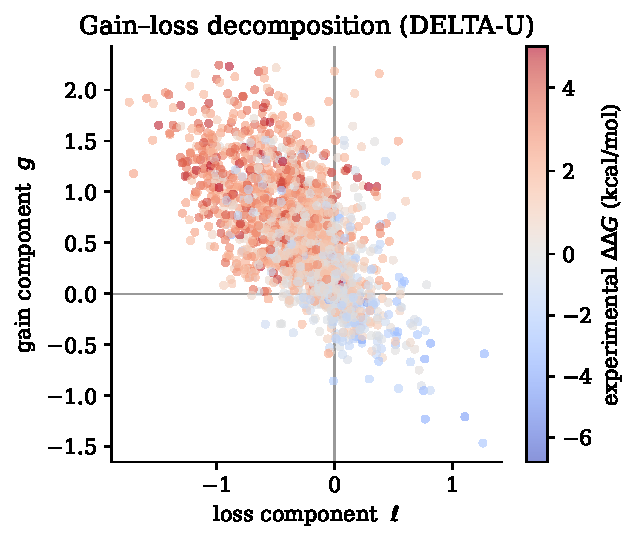
\includegraphics[width=\linewidth]{figures/fig2_gain_loss_scatter.pdf}
\end{minipage}
\hfill
\begin{minipage}{0.48\textwidth}
    \centering
    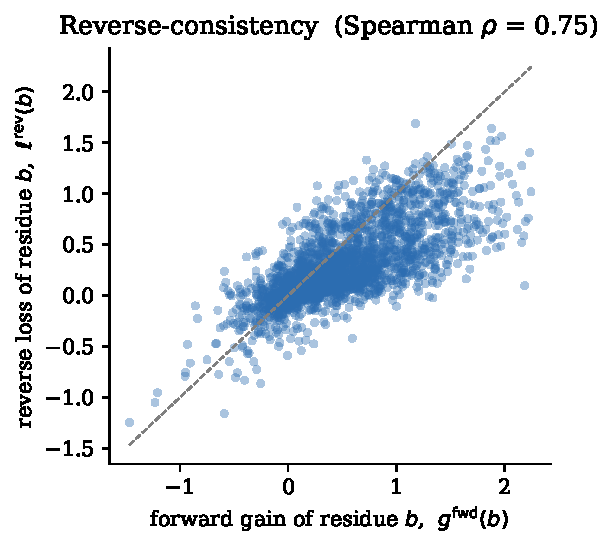
\includegraphics[width=\linewidth]{figures/fig3_reverse_consistency.pdf}
\end{minipage}

\caption{
\textbf{Emergent gain--loss decomposition in DELTA-U.}
(A) Distribution of learned gain and loss components across mutations. Points are colored by experimental $\Delta\Delta G$, showing that stability effects arise from a continuum of gain-loss combinations rather than collapse onto a single branch.
(B) Reverse-consistency diagnostic. The gain assigned to a residue in the forward mutation strongly correlates with the loss assigned to the same residue in the reverse mutation ($\rho=0.75$), indicating that the learned components are anchored to residue identity rather than forming an arbitrary algebraic decomposition.
}
\label{fig:decomposition}
\end{figure*}
\emph{(D2) Conservative-substitution attenuation.} Substitutions between physicochemically similar residues yield a mean component magnitude $|g| + |\ell|$ of $0.47$, against $0.85$ for the remaining substitutions, a ratio of $0.55$. The decomposition thus assigns little gain and little loss precisely where little is chemically exchanged, a regularity that was never encoded in training.

\emph{(D3) Burial association.} The loss component shows a modest but consistent association with wild-type structural burial, with $\rho(|\ell|, \text{contacts}) = 0.41$, exceeding the corresponding value for the gain component, $\rho(|g|, \text{contacts}) = 0.32$ (Figure~\ref{fig:burial}). We are deliberately measured about this result: the separation, while clear, is moderate, and we therefore claim only that the loss component is the more burial-sensitive of the two rather than a clean isolation of the wild-type structural role. Restricting attention to large-hydrophobic-to-small substitutions (the canonical core-packing case) preserves this ordering ($\rho(|\ell|, \text{contacts}) = 0.35$ versus $\rho(|g|, \text{contacts}) = 0.19$ within that subset), indicating it is not an artifact of pooling heterogeneous mutation classes.
\begin{figure*}[t]
\centering
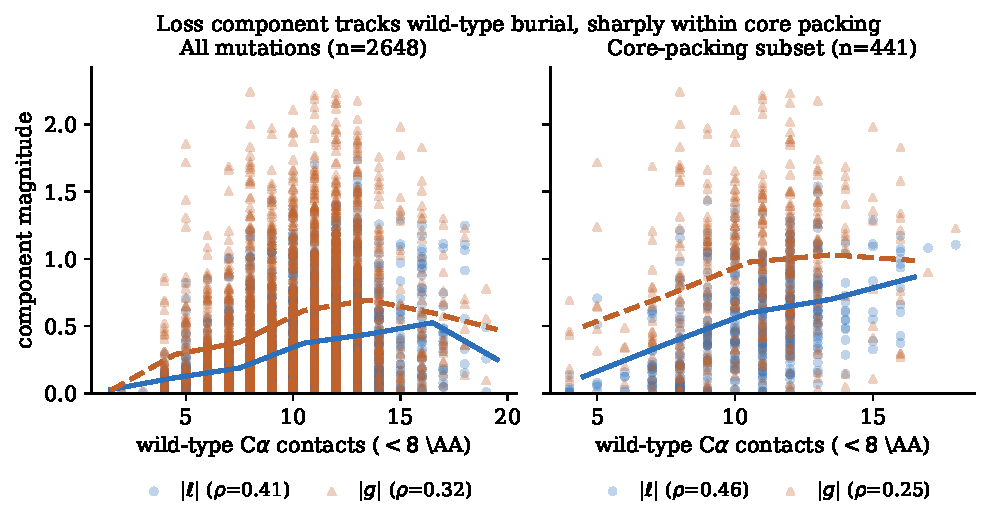
\includegraphics[width=0.9\textwidth]{figures/fig4_burial_merged.pdf}
\caption{
Association between component magnitude and structural burial.
The loss component exhibits stronger burial dependence than the gain component across all mutations.
The separation becomes substantially stronger within core-packing substitutions.
}
\label{fig:burial}
\end{figure*}
\emph{(D4) Embedding directionality.} The learned mutation-type embedding encodes the direction of substitution: a per-channel analysis finds that $58$ of the $64$ latent channels carry anti-symmetric information (mean channelwise anti-symmetry correlation $0.50$), that is, $E_{a,b}$ and $E_{b,a}$ tend toward opposite signs (Figure~\ref{fig:embed}). Direction is thus represented in the model even though only net, direction-paired $\Delta\Delta G$ values were observed during training.
\begin{figure*}[t]
\centering
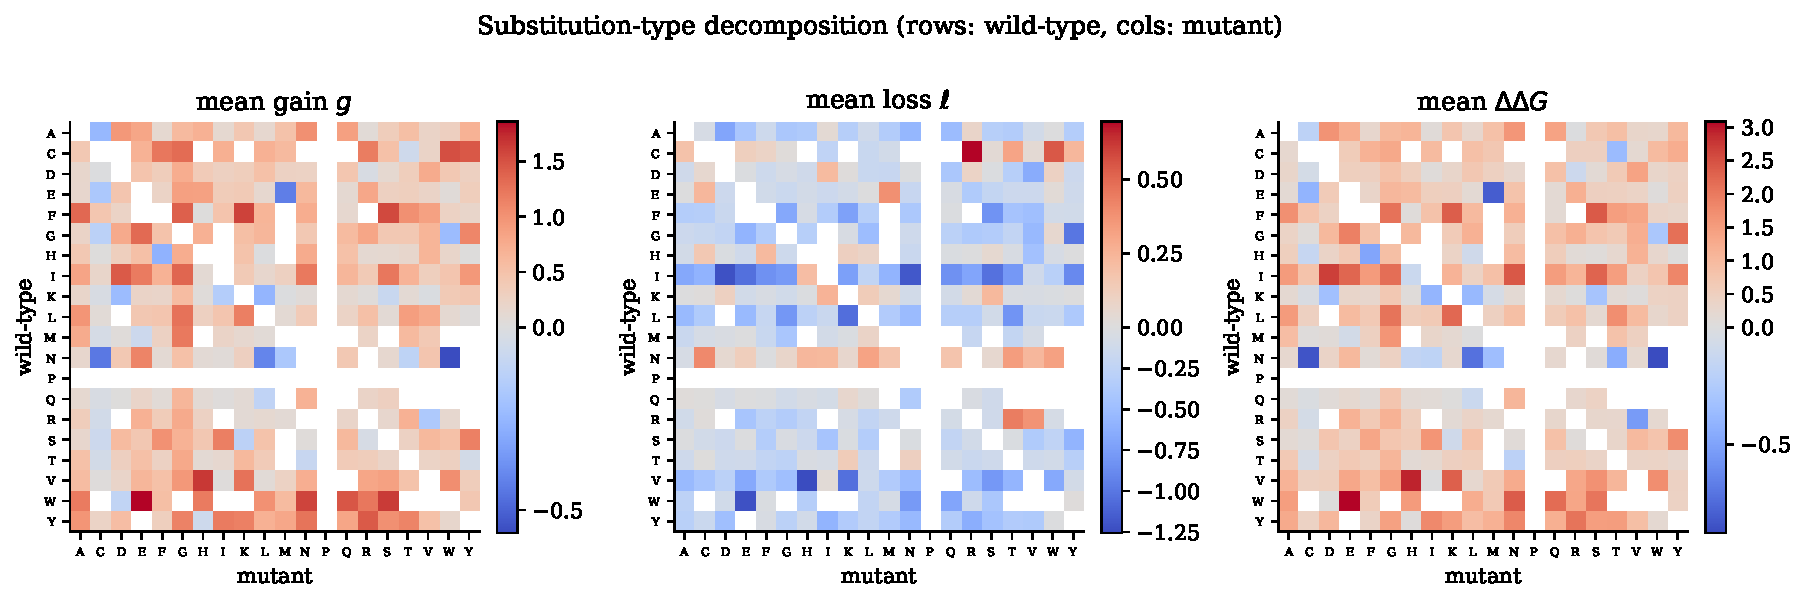
\includegraphics[width=\textwidth]{figures/fig5_mutation_type_heatmaps.pdf}
\caption{
Substitution-specific decomposition.
Rows correspond to wild-type residues and columns to mutant residues.
Mean gain, loss and resulting $\Delta\Delta G$ reveal systematic mutation-type-dependent behavior.
}
\label{fig:embed}
\end{figure*}
Taken together, the four diagnostics indicate that the emergent decomposition is mechanistically consistent and biologically interpretable, while we are careful to claim no recovery of experimentally defined gain and loss, which remain inaccessible to measurement.

\subsection{The decomposition is robust to architectural choice}
\label{sec:robust}
\begin{table}[h]
\centering
\caption{Comparison of DELTA-U and DELTA-B.}
\label{tab:deltablation}
\begin{tabular}{lcc}
\toprule
Metric & DELTA-U & DELTA-B \\
\midrule
Megascale $\rho$ & \textbf{0.675} & 0.667 \\
S669 $\rho$ & \textbf{0.493} & 0.461 \\
Reverse Consistency & 0.754 & \textbf{0.865} \\
Gain Fraction (\%) & 64.6 & \textbf{54.0} \\
Burial Association & \textbf{0.409} & 0.350 \\
Embedding Anti-Symmetry & \textbf{0.50} & 0.06 \\
\bottomrule
\end{tabular}
\end{table}
Comparing DELTA-U with DELTA-B isolated the effect of how the structural context is supplied to the branches (Section~\ref{sec:variants}). The two models are statistically indistinguishable in accuracy, with the best validation Spearman coefficients of $0.741$ and $0.742$, respectively, yet they decompose differently. DELTA-B distributes the prediction more evenly between the branches: the share of destabilization attributed to the gain branch falls from $64.6\%$ in DELTA-U towards a near even $54.0\%$, and reverse consistency rises to $\rho = 0.87$ (from $0.75$). At the same time, the directionality carried by the mutation-type embedding drops sharply, from a mean channelwise anti-symmetry of $0.50$ in DELTA-U ($58/64$ channels) to $0.06$ in DELTA-B ($28/64$ channels). We interpret this as a relocation rather than a loss of information: by conditioning the attention query on residue identity, DELTA-B captures substitution direction in the attention pathway, relieving the embedding of the role. The salient point is that the decomposition,
with its reverse-consistency, conservative attenuation, and burial ordering, emerges under both architectures; what the architecture governs is \emph{how} the decomposition is distributed across the model, not \emph{whether} it arises. This robustness is consistent with the observed regularities reflecting structure in the supervised signal rather than being artifacts of a particular model architecture.

We further note a consistency that spans both models at the level of individual substitution types. The substitutions predicted most accurately and least accurately are largely shared between DELTA-U and DELTA-B: large hydrophobic and charged exchanges (for example, W$\rightarrow$L, A$\rightarrow$Q, A$\rightarrow$K, V$\rightarrow$E) are predicted well by both, whereas substitutions to cysteine (N$\rightarrow$C, S$\rightarrow$C, E$\rightarrow$C) are the hardest for both. The poor performance on cysteine substitutions is independently sensible: the stability effect of introducing a cysteine depends on whether it forms a disulfide bond or remains free, a distinction not determined by the local environment our representation captures. That two architecturally distinct models agree on where the task is easy and where it is hard further supports the view that they are reading shared structure in the data.

\subsection{Burial dependence of the loss component in core-packing substitution}
\label{sec:casestudy}
To test whether the burial association of the loss component reflects a coherent structural signal rather than a pooled-statistics artifact, we isolated the canonical core-packing scenario: substitution of a large hydrophobic wild-type residue (Leu, Ile, Val, Phe, Met, Trp, Tyr) by a smaller residue (Ala, Gly, Ser), the class of mutations whose destabilization is classically attributed to loss of hydrophobic packing and cavity formation. This yields $441$ such mutations in S2648 across structurally diverse proteins, a mechanistically homogeneous subset in which the role of the wild-type residue is well understood.
\begin{figure*}[t]
\centering
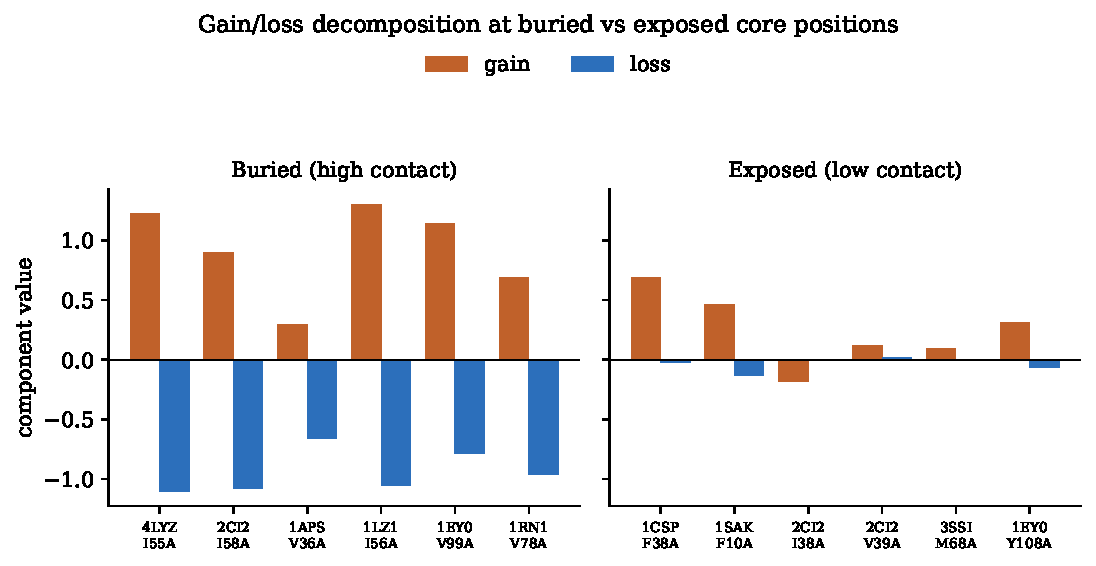
\includegraphics[width=0.9\textwidth]{figures/fig_casestudy_panel.pdf}
\caption{
Representative core-packing substitutions.
Buried mutations exhibit substantially larger loss components than exposed mutations, consistent with disruption of stabilizing packing interactions.
}
\label{fig:casestudy}
\end{figure*}
Within this subset, the separation between the two components is markedly sharper than in the pooled benchmark: the loss component correlates with wild-type burial at $\rho(|\ell|, \text{contacts}) = 0.46$, nearly double the corresponding value for the gain component, $\rho(|g|, \text{contacts}) = 0.26$ (Figures~\ref{fig:burial} and \ref{fig:casestudy}). As the wild-type residue becomes more deeply packed, the decomposition attributes a progressively larger share of the predicted destabilization to the loss term, while the gain term saturates. This is precisely the behavior expected if the loss component captures the removal of stabilizing wild-type contacts: the more contacts the wild-type residue makes, the more there is to lose. We stress that the claim is the burial -\emph{conditional} one visible in the figure, namely that the loss component is preferentially amplified at buried positions; it is not a claim that the loss component uniformly exceeds the gain component in magnitude, which the data do not support.


This subset-level analysis complements the global diagnostics of Section~\ref{sec:diagnostics}: it shows that the burial sensitivity of the loss component, which is modest when measured across all mutation types, becomes pronounced precisely in the mutation class for which core packing is the dominant physical mechanism. We refrain from attributing the effect to named individual mutations, since aligning processed-sequence positions to crystallographic residue numbering and the associated mechanistic literature requires per-structure curation beyond the scope of this analysis; the aggregate, mechanism-homogeneous trend is the evidence we rely on.

\section{Discussion}
DELTA reframes mutation-effect prediction. Rather than treating $\Delta\Delta G$ as a
scalar to be regressed, it treats the prediction as the difference of two latent components and asks what those components, learned without their own supervision, come to represent. The answer, supported by four independent diagnostics, is that they come to behave in a mechanistically consistent manner: direction-anchored across forward and reverse mutations, attenuated for conservative substitutions, modestly burial-sensitive on the loss side, and directionally encoded in the mutation-type embedding. The practical consequence is that a model of this form can supply, alongside each
magnitude, a structured and testable hypothesis about the basis of the predicted effect, which is of direct use in guiding redesign and in prioritizing variants for experimental characterization.

We are explicit about the limits of these claims. First, gain and loss lack experimental ground truth; our evidence is necessarily indirect, resting on internal consistency across independent tests rather than on agreement with measured component values, which do not exist. We therefore describe the components as mechanistically consistent and biologically interpretable, and deliberately avoid asserting that they are physical energies. Second, the burial association, though directionally correct and stable across mutation classes, is modest in magnitude, and we have framed it as such. Third, DELTA's predictive accuracy is competitive with but not superior to a strong single-output backbone; the contribution is the validated decomposition, not a gain in accuracy. Fourth, the anti-symmetry property that our training encourages is established in prior work and is not claimed as a contribution here.

A natural extension is to directly supervise the components against structural quantities, such as burial or packing density, which might sharpen their interpretability. We deliberately do not pursue this, because the central claim of the present work is precisely that mechanistic structure emerges \emph{without} such supervision; introducing component-level labels would make the consistency diagnostics circular and forfeit the result. We therefore record direct physical supervision as
future work whose value would lie in quantifying, by contrast with the present unsupervised setting, how much additional interpretability explicit labels can purchase. Two further directions follow from our findings: the relocation of directional information between the embedding and the attention pathway across DELTA-U and DELTA-B invites a systematic study of where, within a network, such structure is most usefully represented; and the consistent difficulty of cysteine substitutions points to the value of incorporating disulfide-bonding context into the structural representation.
\section{Conclusions}
We posed the change in mutation-induced stability as a latent decomposition problem and asked whether the gain and loss components, which no experiment measures, can be recovered from standard $\Delta\Delta G$ supervision alone. Through DELTA and a suite of held-out diagnostics, we provided evidence that a mechanistically consistent gain-loss decomposition emerges from net supervision without component-level labels; that it is direction-anchored, chemically attenuated, and structurally associated in interpretable ways; and that it arises robustly across two architectural instantiations while preserving the predictive accuracy of a strong single-output backbone. We conclude that mutation-effect models can be designed to yield mechanistic hypotheses alongside scalar predictions, and that the decomposition studied here is a concrete step toward that goal.
\vspace{1.5em}
{
\small
\setlength{\parskip}{0.8em}


\textbf{Author Contributions:}
\textbf{A Shivram:} Conceptualization, Data curation, Methodology, Formal analysis, Investigation, Writing – original draft, Visualization.
\textbf{Aneesh S. Chivukula:} Project administration, Supervision, Software, Validation, Writing – review and editing.
\textbf{Manik Gupta:} Supervision, Resources, Writing – review and editing.
\textbf{Sourav Chowdhury:} Conceptualization, Supervision, Writing – review and editing, Project administration.



\noindent \textbf{Data Availability Statement:} All datasets used in this study are publicly available from their respective sources as described in the Methods section. The source code, trained models, and evaluation scripts required to reproduce the reported results will be made publicly available upon acceptance of the manuscript.


\noindent \textbf{Conflicts of Interest:} The authors declare no conflict of interest.

\par
}

\bibliographystyle{unsrtnat}
\bibliography{reference}

\vspace{2em}
\end{document}